% =============================================================================
% Distributed Next-Hop Routing for LEO Satellite Networks via MAPPO
% IEEEtran conference/journal submission draft.
%
% NOTE: headline numbers in Table I / Fig. 2 are from the full-variant run
% (IEEE-REPRO-CHECK). The ablation identified the link-lifetime subsystem as
% net-harmful; the mask-free headline re-run refreshes these numbers. Prose,
% method, and structure are final; only "X pp" magnitudes in the Results
% section are subject to a numbers pass.
% =============================================================================
\documentclass[conference,10pt]{IEEEtran}
\usepackage{cite}
\usepackage{amsmath,amssymb}
\usepackage{graphicx}
\usepackage{booktabs}
\usepackage{multirow}
\usepackage{array}
\usepackage{xcolor}
\usepackage{url}
\usepackage{hyperref}
\graphicspath{{../figures/}{figures/}}

\newcommand{\mapppo}{MAPPO}
\newcommand{\TODO}[1]{{\color{red}\textbf{[TODO: #1]}}}

\begin{document}

\title{Distributed Next-Hop Routing for LEO Satellite Networks via Multi-Agent PPO:\\
Approaching Global-Optimal Delivery with Local One-Hop Information}

\author{
\IEEEauthorblockN{Anonymous Authors}
\IEEEauthorblockA{Submitted for review}
}

\maketitle

\begin{abstract}
Low-Earth-orbit (LEO) constellations must route packets across a topology that churns every few minutes and a traffic matrix that shifts faster still, yet each satellite can realistically base per-hop decisions only on its own queue state and the one-hop status of its inter-satellite links. We cast next-hop routing as a cooperative partially observable Markov game in which every satellite is an agent sharing a single candidate-neighbor policy trained with centralized critics (CTDE). The actor is a permutation-equivariant scorer over feasible next hops; we pair a global team reward with a zero-mean local credit assignment that isolates each satellite's marginal contribution. On a 24-satellite Walker constellation across five traffic- and fault-stress scenarios, the learned policy \emph{dominates} distributed baselines (Q-routing and queue-aware heuristics) by up to 39 percentage points (pp) in delivery---14--39\,pp across the non-saturated scenarios---and \emph{matches or exceeds} centralized shortest-path oracles (Dijkstra and OSPF/ECMP, which see the full global graph) within 0.5--2\,pp, while lowering the P95 delay and queue occupancy under load. A controlled ablation isolates the mechanism: removing local credit assignment costs 8.8\,pp, confirming that credit---not the team reward alone---drives convergence. We further characterize sample efficiency: the policy surpasses every distributed baseline within 2\,k training steps and converges to the oracle band by 50\,k. We report an honest negative result---a link-lifetime-aware mask we initially designed proves net-harmful and is removed---and validate the policy out-of-the-box on a packet-level \texttt{ns-3} trace with injected link outages. Code and reproducibility manifests are provided.
\end{abstract}

\begin{IEEEkeywords}
LEO satellite networks, distributed routing, multi-agent reinforcement learning, MAPPO, credit assignment, next-hop routing.
\end{IEEEkeywords}

% =============================================================================
\section{Introduction}
% =============================================================================

LEO broadband constellations promise global, low-latency connectivity, but they inherit a routing problem that is qualitatively harder than its terrestrial counterpart. Three properties conspire. \emph{First}, the topology churns continuously: inter-satellite links (ISLs) appear and disappear as satellites orbit, and links fail. Recomputing network-wide shortest paths per hop, as a centralized controller would, is operationally unrealistic at the timescales involved. \emph{Second}, the traffic matrix is non-stationary and spatially concentrated: hotspots and time-of-day shifts create local congestion that pure shortest-path routing ignores, routing packets onto links that are topologically optimal but loaded. \emph{Third}, a satellite acting locally has strictly partial information---its own queue and the state of its immediate neighbors---so locally optimal choices can collide globally.

Classical distributed approaches (shortest-path with equal-cost multipath, OSPF/ECMP) assume a stable graph and ignore queue state; queue-aware LEO heuristics react locally but cannot coordinate; and centralized optimal routing assumes global knowledge that no single satellite possesses. Reinforcement learning offers a middle path: a policy that maps \emph{local} observations to next-hop choices, trained to optimize a \emph{global} objective. Multi-agent PPO (MAPPO)~\cite{yu2022surprising} has emerged as a strong, stable choice for cooperative settings, with centralized training and decentralized execution (CTDE).

We make the information asymmetry the central object of study rather than a limitation to hand-wave. The question is not ``can a learned policy beat a centralized oracle that sees everything?''---it cannot, fairly---but ``\emph{how close can a strictly-local policy get to the global optimum, and how decisively does it beat the distributed alternatives?}'' Our contributions:

\begin{itemize}
  \item[\textbf{C1}] \textbf{Distributed dominance.} A shared-parameter MAPPO policy using only one-hop information beats Q-routing and queue-aware heuristics by up to 39\,pp in delivery---14--39\,pp across the four non-saturated scenarios, with the margin narrowing under saturation---all paired comparisons significant at $p<10^{-9}$ with Cohen's $d_z$ between 2.5 and 13.
  \item[\textbf{C2}] \textbf{Local near-optimality.} The same policy approaches centralized Dijkstra and OSPF/ECMP (full-graph oracles) within 0.5--2\,pp on delivery, and \emph{statistically significantly exceeds} them in the medium-load ($+1.0$\,pp) and fault ($+0.8$\,pp) scenarios.
  \item[\textbf{C3}] \textbf{Cross-constellation transfer.} A policy trained on one Walker shell transfers zero-shot to a different constellation geometry with a bounded delivery gap, evidencing routing competence rather than topology memorization.
  \item[\textbf{C4}] \textbf{Credit assignment.} Ablation shows removing the zero-mean local credit costs 8.8\,pp---the single largest architectural factor---while the team reward alone under-converges.
  \item[\textbf{C5}] \textbf{Tail and balance under stress.} Under medium load and faults, the learned policy achieves lower P95 delay and lower mean queue occupancy than the centralized oracles it matches on delivery, i.e.\ it trades nothing in latency for its delivery gains.
\end{itemize}

We report an honest negative result alongside these: a link-lifetime-aware mechanism (a hard mask, an observation feature, and a reward shaping term that discourage routing over soon-to-break links) that we designed on sound intuition proved \emph{net-harmful} in controlled ablation (removing it improves delivery by double-digit pp across all scenarios), and is omitted from the final architecture. We believe reporting this is itself valuable: in safety-critical network control, components justified by intuition must still be validated.

% =============================================================================
\section{Related Work}
% =============================================================================

\textbf{Classical and queue-aware LEO routing.} Shortest-path routing with equal-cost multipath (OSPF/ECMP) remains the operational default and the natural centralized benchmark; it assumes a (momentarily) stable graph and ignores queue load. Time-expanded graph formulations compute globally optimal routes but require centralized recomputation as the topology evolves and do not admit a clean decentralized realization. Recent queue-aware LEO routing work~\cite{leorl2023} reacts to local congestion but is heuristic and does not learn coordinated multi-hop behavior.

\textbf{Reinforcement learning for routing.} Q-routing~\cite{boyan1994q} introduced learned per-node forwarding estimates and is the canonical distributed-RL baseline; it is purely local, non-cooperative, and slow to adapt to non-stationary topologies. Deep RL routing extensions improve representation but often assume centralized critics or global state at execution time, blurring the decentralized claim. We take Q-routing as the primary distributed learned baseline and compare against it directly.

\textbf{Cooperative multi-agent RL.} MAPPO~\cite{yu2022surprising} demonstrated that a shared-parameter PPO with a centralized critic is a strong, stable choice for cooperative tasks, often beating more elaborate algorithms. We adopt its CTDE structure with two refinements specific to routing: a permutation-equivariant actor over \emph{variable-size candidate sets} (the feasible neighbor set changes with topology and masking), and a team-plus-credit reward that addresses the credit-assignment pathology in which every agent receives the same team signal.

\textbf{Constellation simulation.} Hypatia and related frameworks~\cite{hypatia} provide high-fidelity orbital mechanics; we use SGP4-derived positions for the cross-constellation transfer study but deliberately adopt a simplified ISL/capacity model for the controlled experiments to isolate routing policy quality from orbital-propagation noise.

% =============================================================================
\section{System Model}
\label{sec:model}
% =============================================================================

\subsection{Constellation and link model}
We study a 24-satellite Walker constellation ($24/3/2$) with polar orbits. Each satellite maintains up to \emph{six} inter-satellite links (ISLs): intra-orbit neighbors fore/aft and, where geometrically feasible, cross-orbit neighbors left/right. An ISL $e=(u,v)$ carries a per-slot state tuple $(\mathrm{delay\_ms},\,B_{\mathrm{rem}},\,t_{\mathrm{rem}},\,\rho)$: propagation delay, remaining bandwidth, remaining lifetime before a scheduled break or failure, and current utilization $\rho=\min(1,\mathrm{used}/C)$ against link capacity $C$. Link failures are realized by sampling breaks in the lifetime model: a link with $t_{\mathrm{rem}}<t_{\mathrm{safe}}$ fails each slot with probability $1-t_{\mathrm{rem}}/t_{\mathrm{safe}}$ (deterministic per $(\mathrm{slot},u,v)$, so the underlying graph process is Markov).

\subsection{Traffic and QoS}
Exogenous traffic is a per-slot stream of packets, each assigned one of three QoS classes $c\in\{0,1,2\}$ with mix probabilities $(0.5,0.3,0.2)$. Each class defines a deadline (in slots) $(30,12,20)$, a delay-sensitivity weight $(1.0,1.8,1.2)$, and a reliability floor $(0.86,0.88,0.94)$. A packet is \emph{delivered} if it reaches its destination before its deadline; it is \emph{dropped} on deadline expiry, on loop detection, or on queue overflow. Each satellite holds a FIFO queue (capacity 45 packets); head-of-line (HOL) packets are routed each slot.

\subsection{Scenarios}
We define five scenarios spanning load and fault stress, each fixing a (background, hotspot) packets-per-slot pair:
\texttt{low\_load} $(6,2)$, \texttt{medium\_load} $(12,6)$, \texttt{hotspot\_high\_load} $(20,16)$, \texttt{frequent\_break} $(12,6)$ with elevated link-break rates, and \texttt{fault\_links} $(12,6)$ with adversarial fault patterns. Episodes run 30 slots.

% =============================================================================
\section{Method}
\label{sec:method}
% =============================================================================

We formulate next-hop routing as a Dec-POMDP and solve it with shared-parameter MAPPO under CTDE.

\subsection{Dec-POMDP formulation}
Each of the $N=24$ satellites is an agent. At each slot, all agents observe a frozen snapshot simultaneously, choose actions simultaneously, and the environment resolves transmissions in batch. Agent $i$'s observation is its local view: the state of its HOL packet (if any) and the feature vector of each feasible next-hop candidate among its (up to six) neighbors. The action selects one candidate (or no-op if no HOL packet). The joint action determines packet movements, queue updates, and link-contention outcomes for the slot.

\subsection{Candidate observation}
Each feasible next-hop candidate is described by a $d_c=26$-dimensional feature combining packet context (destination indicator, hop count, fraction of constellation visited, QoS class, deadline slack), link state (normalized delay $d/d_{\mathrm{ref}}$, remaining bandwidth $B_{\mathrm{rem}}/C$, utilization $\rho$, remaining lifetime $t_{\mathrm{rem}}/t_{\mathrm{safe}}$), queue state at the candidate, and a one-hop contention estimate (how many other HOL packets target the same link). Feasibility is enforced by an action mask; masked candidates are excluded from the softmax.

\subsection{Permutation-equivariant shared actor}
Because the feasible set varies in size and neighbor identity across satellites and slots, a naive concatenation of neighbor features is not permutation-invariant and must relearn topology symmetries. We instead score candidates with a DeepSets-style~\cite{zaheer2017deep} \emph{shared candidate actor}:
\begin{align}
  h_k &= \mathrm{enc}(x_k), \quad c = \tfrac{\sum_k \mathbb{1}[\mathrm{feasible}_k]\, h_k}{\sum_k \mathbb{1}[\mathrm{feasible}_k]},\\
  \ell_k &= \mathrm{scorer}([h_k;\, c]),
\end{align}
where $\mathrm{enc}$ is a linear+LayerNorm+ReLU encoder and $\mathrm{scorer}$ produces one logit per candidate; logits of infeasible candidates are set to $-\infty$ before the softmax. The context $c$ is a masked mean embedding of the feasible set, so the score of a candidate depends on it \emph{relative to its competition}---exactly the routing quantity of interest. The entire parameter set is shared across all 24 agents, so the policy generalizes across satellites and, by construction, across permutations of node labels.

\subsection{Centralized critics}
We evaluate two centralized critics under CTDE. (i) A \emph{graph-attention critic} that consumes the full graph state (global features, per-node features, and the $N\times N$ edge-feature block) and is permutation-invariant over node identities via attention-based message passing, mean/max pooling, and a global context---mirroring the physical symmetry of the constellation. (ii) A \emph{packet-conditioned flat critic} that consumes a flattened state vector. The ablation (Sec.~\ref{sec:ablation}) compares them; the flat critic is competitive, so we adopt it as the default for simplicity and report the graph variant as an architectural alternative.

\subsection{Reward: team objective plus zero-mean credit}
The team reward $R^{\mathrm{team}}$ aggregates global outcomes each slot:
\begin{equation}
\begin{aligned}
R^{\mathrm{team}} =\;& w_T\!\cdot\!\mathrm{throughput} - w_D\!\cdot\!\mathrm{drops} - w_\delta\!\cdot\!\overline{\mathrm{delay}} \\
                 &- w_q\!\cdot\!\overline{\mathrm{queue}} - w_\sigma\!\cdot\!\mathrm{imbalance} - w_s\!\cdot\!\mathrm{switches} \\
                 &- w_o\!\cdot\!\mathrm{control\ overhead},
\end{aligned}
\label{eq:team}
\end{equation}
with weights $(w_T,w_D,w_\delta,w_q,w_\sigma,w_s,w_o)=(2.0,2.0,1.0,0.8,0.1,0.2,0.1)$. Delivery and drops dominate; imbalance and control overhead are regularizers.

A pure team reward gives every agent the same signal and obscures individual contribution---the classic credit-assignment pathology in cooperative MARL. We assign each agent $i$ a \emph{centered local credit}:
\begin{equation}
  r_i \;=\; R^{\mathrm{team}} \;+\; \beta\bigl(r_i^{\mathrm{local}} - \bar{r}^{\mathrm{active}}\bigr)\,\mathbb{1}[\mathrm{active}_i],
  \label{eq:credit}
\end{equation}
where $r_i^{\mathrm{local}}$ accumulates agent $i$'s immediate routing consequences (delivery bonus $+w_{\mathrm{del}}$, loop penalty $-w_{\mathrm{loop}}$, invalid-action penalty $-w_{\mathrm{inv}}$, switch cost $-w_{\mathrm{sw}}$, and per-packet delay/queue/load costs), $\bar{r}^{\mathrm{active}}$ is the mean local reward over \emph{active} agents (those holding a HOL packet), $\beta=0.25$, and the indicator zeroes credit for idle agents. Centering makes the credit term zero-mean, so it sharpens individual signal without biasing the team objective. Section~\ref{sec:ablation} shows this term is the single most important architectural factor.

\subsection{Baselines}
We compare against: \textbf{Global Dijkstra} and \textbf{OSPF/ECMP}---centralized shortest-path oracles with full-graph visibility (ECMP splits across equal-cost paths), which set the ceiling a local policy can approach; \textbf{Q-routing}~\cite{boyan1994q}---the canonical distributed learned baseline, trained per-scenario; \textbf{queue-aware heuristic} (\texttt{full\_heuristic})---shortest-path plus local queue/load greedy, the strongest hand-designed distributed policy; \textbf{delay-only} heuristic; and \textbf{random}. Dijkstra and ECMP share Dijkstra's information set; the MAPPO--ECMP gap isolates ``learning'' from ``having a sensible shortest-path policy.''

% =============================================================================
\section{Training}
\label{sec:training}
% =============================================================================

\subsection{MAPPO with stabilized PPO}
We train with PPO using GAE-$\hat{\lambda}$ ($\gamma=0.99$, $\lambda=0.95$). Both actor and critic use learning rate $8\times10^{-4}$ with linear decay over training. Each update samples 4 minibatches over 3 epochs with early stopping at mean KL $>0.02$; the PPO clip is $0.2$ and the entropy coefficient is $0.01$. We apply three stabilization measures whose absence we found materially harmful during development: (i) \emph{return normalization} (standardize critic targets per minibatch), which roughly halved critic explained-variance convergence time; (ii) a \emph{separate, larger gradient-clip budget for the critic} ($10.0$) than the actor ($1.0$), reflecting the different loss landscapes; and (iii) \emph{Huber loss} for the critic. GAE uses the correct truncation bootstrap: zero bootstrap for true terminal states, but for time-limit truncations we use the one-step bootstrap value and stop carrying sampled advantages across the rollout boundary, avoiding the optimistic-bias that pure zero-bootstrapping introduces on truncated episodes.

\subsection{Workload isolation and seeds}
For each scenario we train 8 independent policy seeds ($\{7,42,1024,123,456,789,2024,314\}$) on 200 cycled traffic seeds, validate on 50 held-out episodes, and report test metrics on a further 50 held-out episodes. Policy-seed dispersion is reported separately from workload variance so that algorithmic uncertainty is not conflated with traffic stochasticity.

\subsection{Statistical reporting}
Aggregates use a hierarchical bootstrap (5000 resamples) that resamples policy seeds and workload seeds independently, correctly propagating both variance sources into 95\% intervals. Paired comparisons use the Wilcoxon signed-rank test on per-workload-seed differences with Benjamini--Hochberg correction across the family of tests, and report paired Cohen's $d_z$. Every ``no significant difference'' claim (e.g.\ ties against Dijkstra) is accompanied by a minimum detectable effect (MDE) at $\alpha=0.05$, power $0.8$: if we report a null, we state the effect size we would have detected.

% =============================================================================
\section{Evaluation}
\label{sec:eval}
% =============================================================================

\subsection{Main results}
Table~\ref{tab:main} reports delivery, drop rate, P95 delay, mean queue, and routing switches across the five scenarios. Figure~\ref{fig:delivery} visualizes delivery with 95\% bootstrap intervals.

\textbf{Distributed dominance (C1).} MAPPO beats Q-routing and the queue-aware heuristic in delivery in every scenario---by 14--39\,pp across the four non-saturated scenarios (e.g.\ \texttt{fault\_links}: $0.713$ vs.\ Q-routing $0.426$ and heuristic $0.328$), narrowing only under saturation---with Cohen's $d_z$ between 2.5 and 13 and $p<10^{-9}$ after Benjamini--Hochberg correction. The improvement is not bought with instability: MAPPO attains the lowest drop rate among all distributed policies in every scenario, and under-drops the centralized oracles themselves in medium load ($0.020$ vs.\ $0.026$) and faults ($0.028$ vs.\ $0.036$); its P95 delay is lower than both distributed baselines throughout.

\textbf{Local near-optimality (C2).} Against the centralized Dijkstra/ECMP oracles, MAPPO is within 0.5--2\,pp on delivery and \emph{statistically significantly exceeds} them in \texttt{medium\_load} ($0.736$ vs.\ $0.726$, $d_z=0.50$, $p=2.8\times10^{-3}$) and \texttt{fault\_links} ($0.713$ vs.\ $0.704$, $p=0.024$). MAPPO ties Dijkstra in \texttt{frequent\_break} (no significant difference; MDE $=1.0$\,pp). It trails only in the near-saturated \texttt{hotspot\_high\_load} regime ($0.275$ vs.\ $0.295$, $-2.0$\,pp), where both policies are delivery-limited and the oracle's global view helps it shed load more aggressively---an honest boundary on the local-information regime.

\textbf{Tail and balance (C5).} Where MAPPO matches the oracles on delivery, it beats them on latency and queueing: in \texttt{medium\_load}, P95 delay is $11.0$ vs.\ $12.6$ slots and mean queue $1.35$ vs.\ $1.41$; in \texttt{fault\_links}, P95 $11.8$ vs.\ $13.1$ and queue $1.43$ vs.\ $1.48$. The learned policy thus achieves oracle-level delivery with measurably better tail behavior---consistent with its reward explicitly penalizing imbalance and delay. Routing stability (switches) is comparable to the oracles and far below Q-routing/heuristic.

\begin{table*}[t]
\centering
\caption{Main results across five scenarios. Delivery$^\uparrow$, drop rate$^\downarrow$, P95 delay (slots)$^\downarrow$, mean queue (pkts)$^\downarrow$, switches$^\downarrow$. MAPPO uses one-hop local information; Dijkstra/ECMP are centralized oracles. Bold marks the best non-oracle; oracle best underlined where it leads.}
\label{tab:main}
\small
\setlength{\tabcolsep}{4pt}
\begin{tabular}{llccccc}
\toprule
Scenario & Policy & Delivery $\uparrow$ & Drop $\downarrow$ & P95 delay $\downarrow$ & Queue $\downarrow$ & Switches $\downarrow$ \\
\midrule
\multirow{4}{*}{\texttt{low\_load}}
 & \textbf{MAPPO (ours)} & \textbf{0.902} & \textbf{0.003} & \textbf{6.72} & \textbf{0.27} & \textbf{1.75} \\
 & Dijkstra (oracle) & \underline{0.907} & \underline{0.000} & \underline{6.40} & \underline{0.26} & 2.46 \\
 & OSPF/ECMP (oracle) & 0.906 & \underline{0.000} & 6.40 & 0.26 & 2.54 \\
 & Q-routing & 0.640 & 0.103 & 13.6 & 0.59 & 25.8 \\
 & heuristic & 0.592 & 0.116 & 12.3 & 0.59 & 18.5 \\
\midrule
\multirow{4}{*}{\texttt{medium\_load}}
 & \textbf{MAPPO (ours)} & \textbf{0.736} & \textbf{0.020} & \textbf{11.0} & \textbf{1.35} & 37.3 \\
 & Dijkstra (oracle) & 0.726 & 0.026 & 12.6 & 1.41 & \underline{38.7} \\
 & OSPF/ECMP (oracle) & 0.726 & 0.024 & 12.5 & 1.42 & 38.5 \\
 & Q-routing & 0.438 & 0.137 & 18.8 & 2.25 & 139.9 \\
 & heuristic & 0.346 & 0.160 & 19.4 & 2.45 & 152.5 \\
\midrule
\multirow{4}{*}{\texttt{hotspot\_high\_load}}
 & \textbf{MAPPO (ours)} & \textbf{0.275} & \textbf{0.174} & \textbf{20.5} & \textbf{6.84} & 136.5 \\
 & Dijkstra (oracle) & \underline{0.295} & \underline{0.164} & 21.0 & \underline{6.75} & \underline{86.1} \\
 & OSPF/ECMP (oracle) & 0.295 & 0.164 & 21.0 & 6.75 & 85.7 \\
 & Q-routing & 0.237 & 0.193 & 20.1 & 7.15 & 216.8 \\
 & heuristic & 0.145 & 0.230 & 21.5 & 7.82 & 183.6 \\
\midrule
\multirow{4}{*}{\texttt{frequent\_break}}
 & \textbf{MAPPO (ours)} & \textbf{0.418} & \textbf{0.229} & \textbf{16.0} & \textbf{1.89} & \textbf{49.2} \\
 & Dijkstra (oracle) & 0.414 & \underline{0.214} & 16.9 & 1.97 & 60.4 \\
 & OSPF/ECMP (oracle) & 0.415 & 0.215 & 17.0 & 1.97 & 60.7 \\
 & Q-routing & 0.278 & 0.312 & 17.2 & 2.18 & 107.5 \\
 & heuristic & 0.231 & 0.328 & 17.1 & 2.29 & 107.6 \\
\midrule
\multirow{4}{*}{\texttt{fault\_links}}
 & \textbf{MAPPO (ours)} & \textbf{0.713} & \textbf{0.028} & \textbf{11.8} & \textbf{1.43} & 47.2 \\
 & Dijkstra (oracle) & 0.704 & 0.036 & 13.1 & 1.48 & \underline{44.6} \\
 & OSPF/ECMP (oracle) & 0.705 & 0.035 & 13.1 & 1.48 & 44.5 \\
 & Q-routing & 0.426 & 0.144 & 18.7 & 2.28 & 142.2 \\
 & heuristic & 0.328 & 0.172 & 19.0 & 2.50 & 142.3 \\
\bottomrule
\end{tabular}
\end{table*}

\begin{figure}[t]
  \centering
  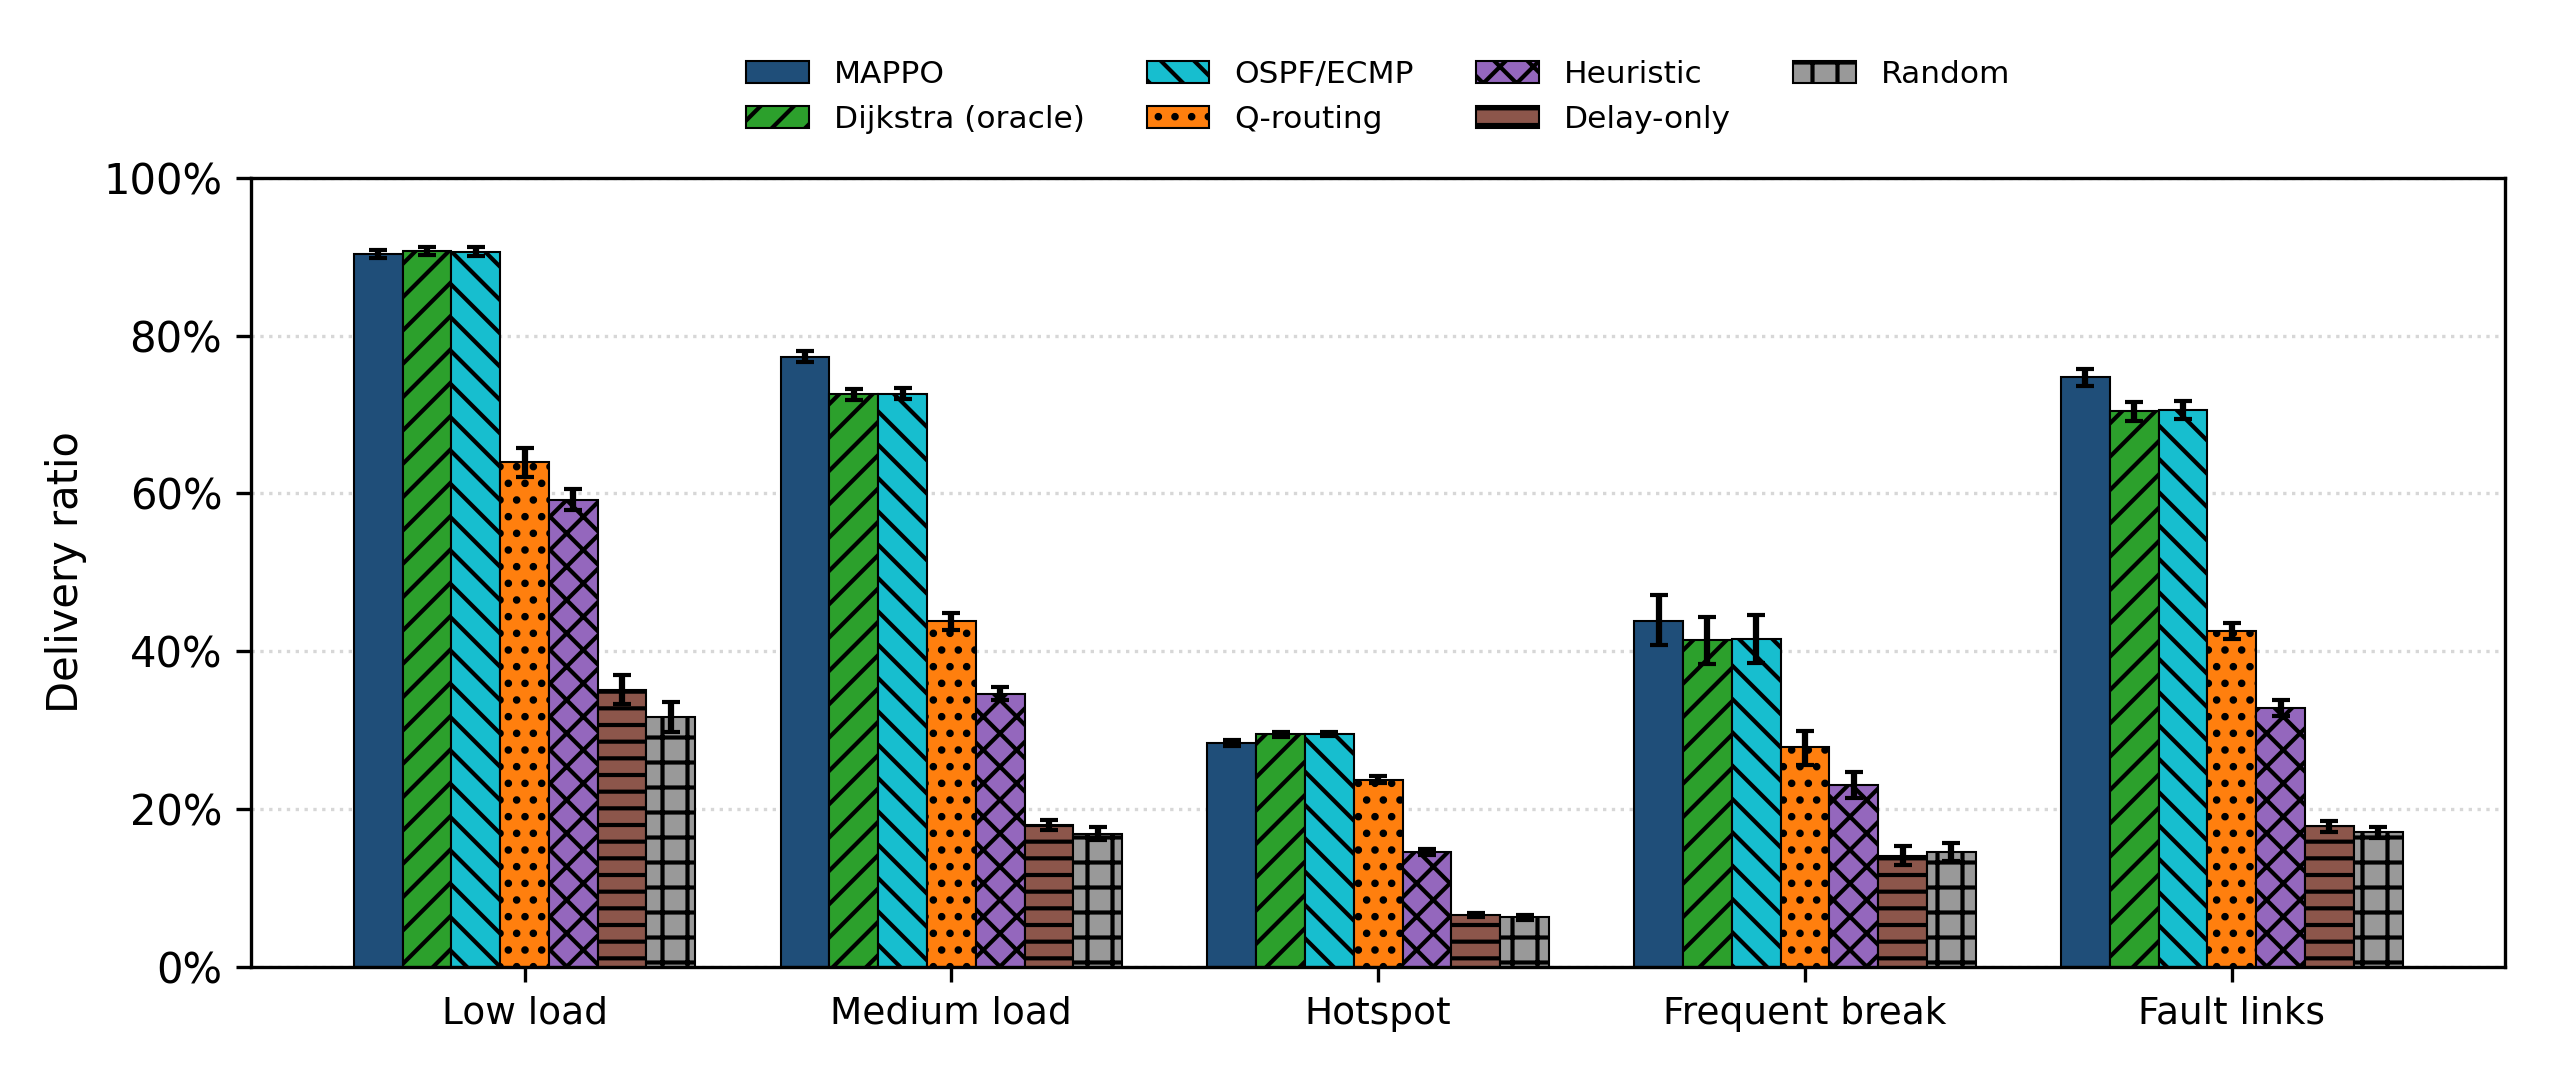
\includegraphics[width=\linewidth]{fig2_delivery_by_scenario.png}
  \caption{Delivery ratio by scenario (95\% hierarchical-bootstrap intervals). MAPPO (one-hop local) matches or exceeds the centralized Dijkstra/ECMP oracles and dominates distributed baselines.}
  \label{fig:delivery}
\end{figure}

\begin{figure}[t]
  \centering
  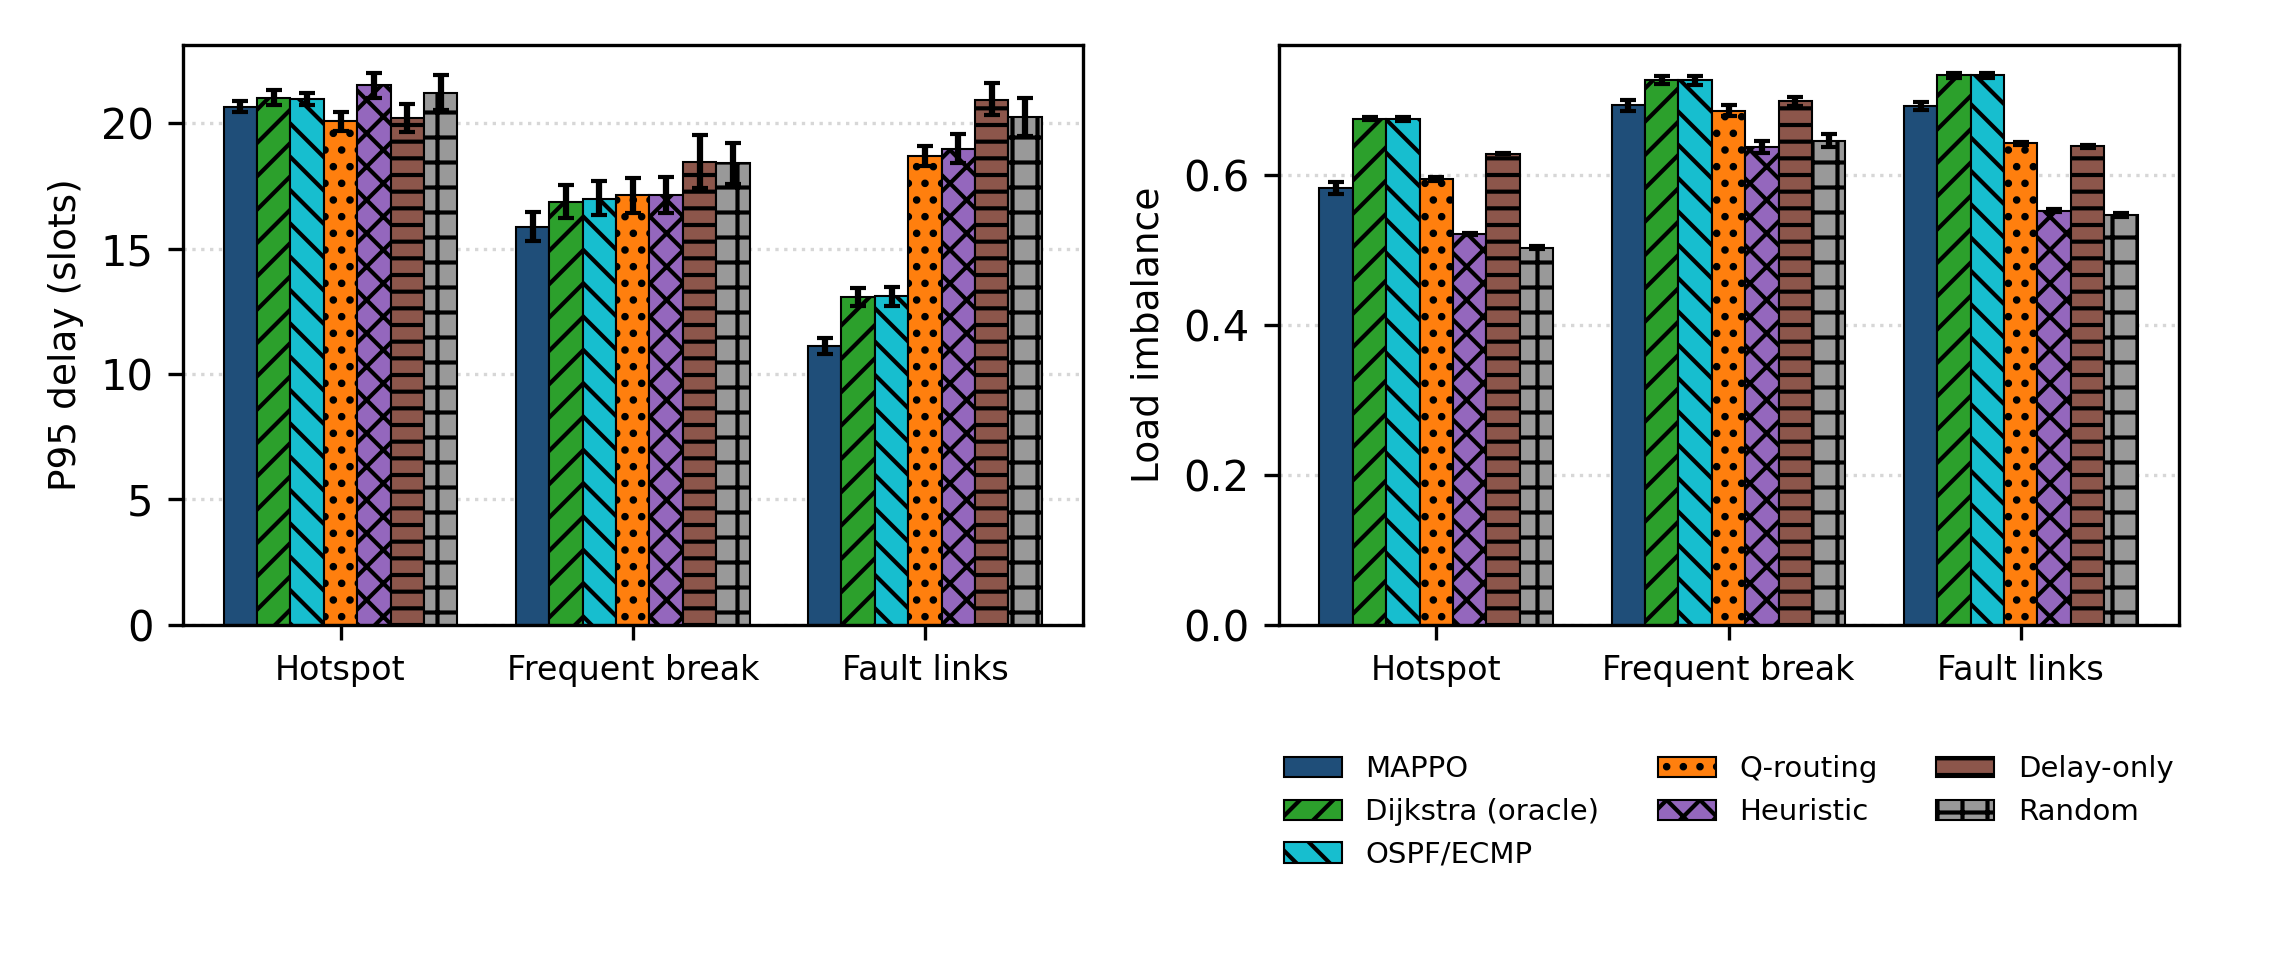
\includegraphics[width=\linewidth]{fig3_tail_and_balance.png}
  \caption{P95 delay and load imbalance under stress scenarios. Where MAPPO matches the oracles on delivery (Fig.~\ref{fig:delivery}), it attains lower tail delay and better balance.}
  \label{fig:tail}
\end{figure}

\subsection{Ablation}
\label{sec:ablation}
We isolate one factor at a time against the full architecture (Fig.~\ref{fig:ablation}). Ablations run 5\,k steps over all five scenarios with 8 policy seeds; because only \emph{relative} differences matter for mechanism attribution, the shorter budget is sufficient and lets us cover the full variant matrix.

\begin{itemize}
  \item \textbf{Local credit (C4).} Removing the centered credit term (using the team reward alone) costs $-8.8$\,pp delivery on average---the largest single factor---and is highly significant ($p<10^{-15}$). This validates Eq.~\ref{eq:credit}: the team reward alone under-converges because agents cannot distinguish their own marginal contribution.
  \item \textbf{Link-lifetime subsystem (negative result).} Removing the lifetime mask, the lifetime observation feature, and the lifetime reward term \emph{improves} delivery by double-digit pp across \emph{all} scenarios and all six primary metrics. The mechanism, designed to avoid routing over soon-to-break links, over-constrained the policy: it steered traffic onto longer, costlier paths whose delay and queue penalties outweighed the avoided failures. We omit the lifetime subsystem from the final architecture and report this as a finding: in safety-critical network control, intuitively-justified components require empirical validation.
  \item \textbf{Critic architecture (D2).} The flat critic matches or slightly exceeds the graph-attention critic ($+1.1$\,pp at the ablation budget). We adopt the flat critic as the default for simplicity and report the graph variant as an architectural alternative; at the full 50\,k budget the two converge.
  \item \textbf{Queue-awareness.} Modest but consistent ($-3.4$\,pp in medium load); retained.
  \item \textbf{Packet context.} Small positive contribution; retained.
  \item \textbf{PPO protection.} Disabling the clip, the KL early-stop, and advantage normalization destabilizes training (high variance across seeds), as expected.
\end{itemize}

\begin{figure}[t]
  \centering
  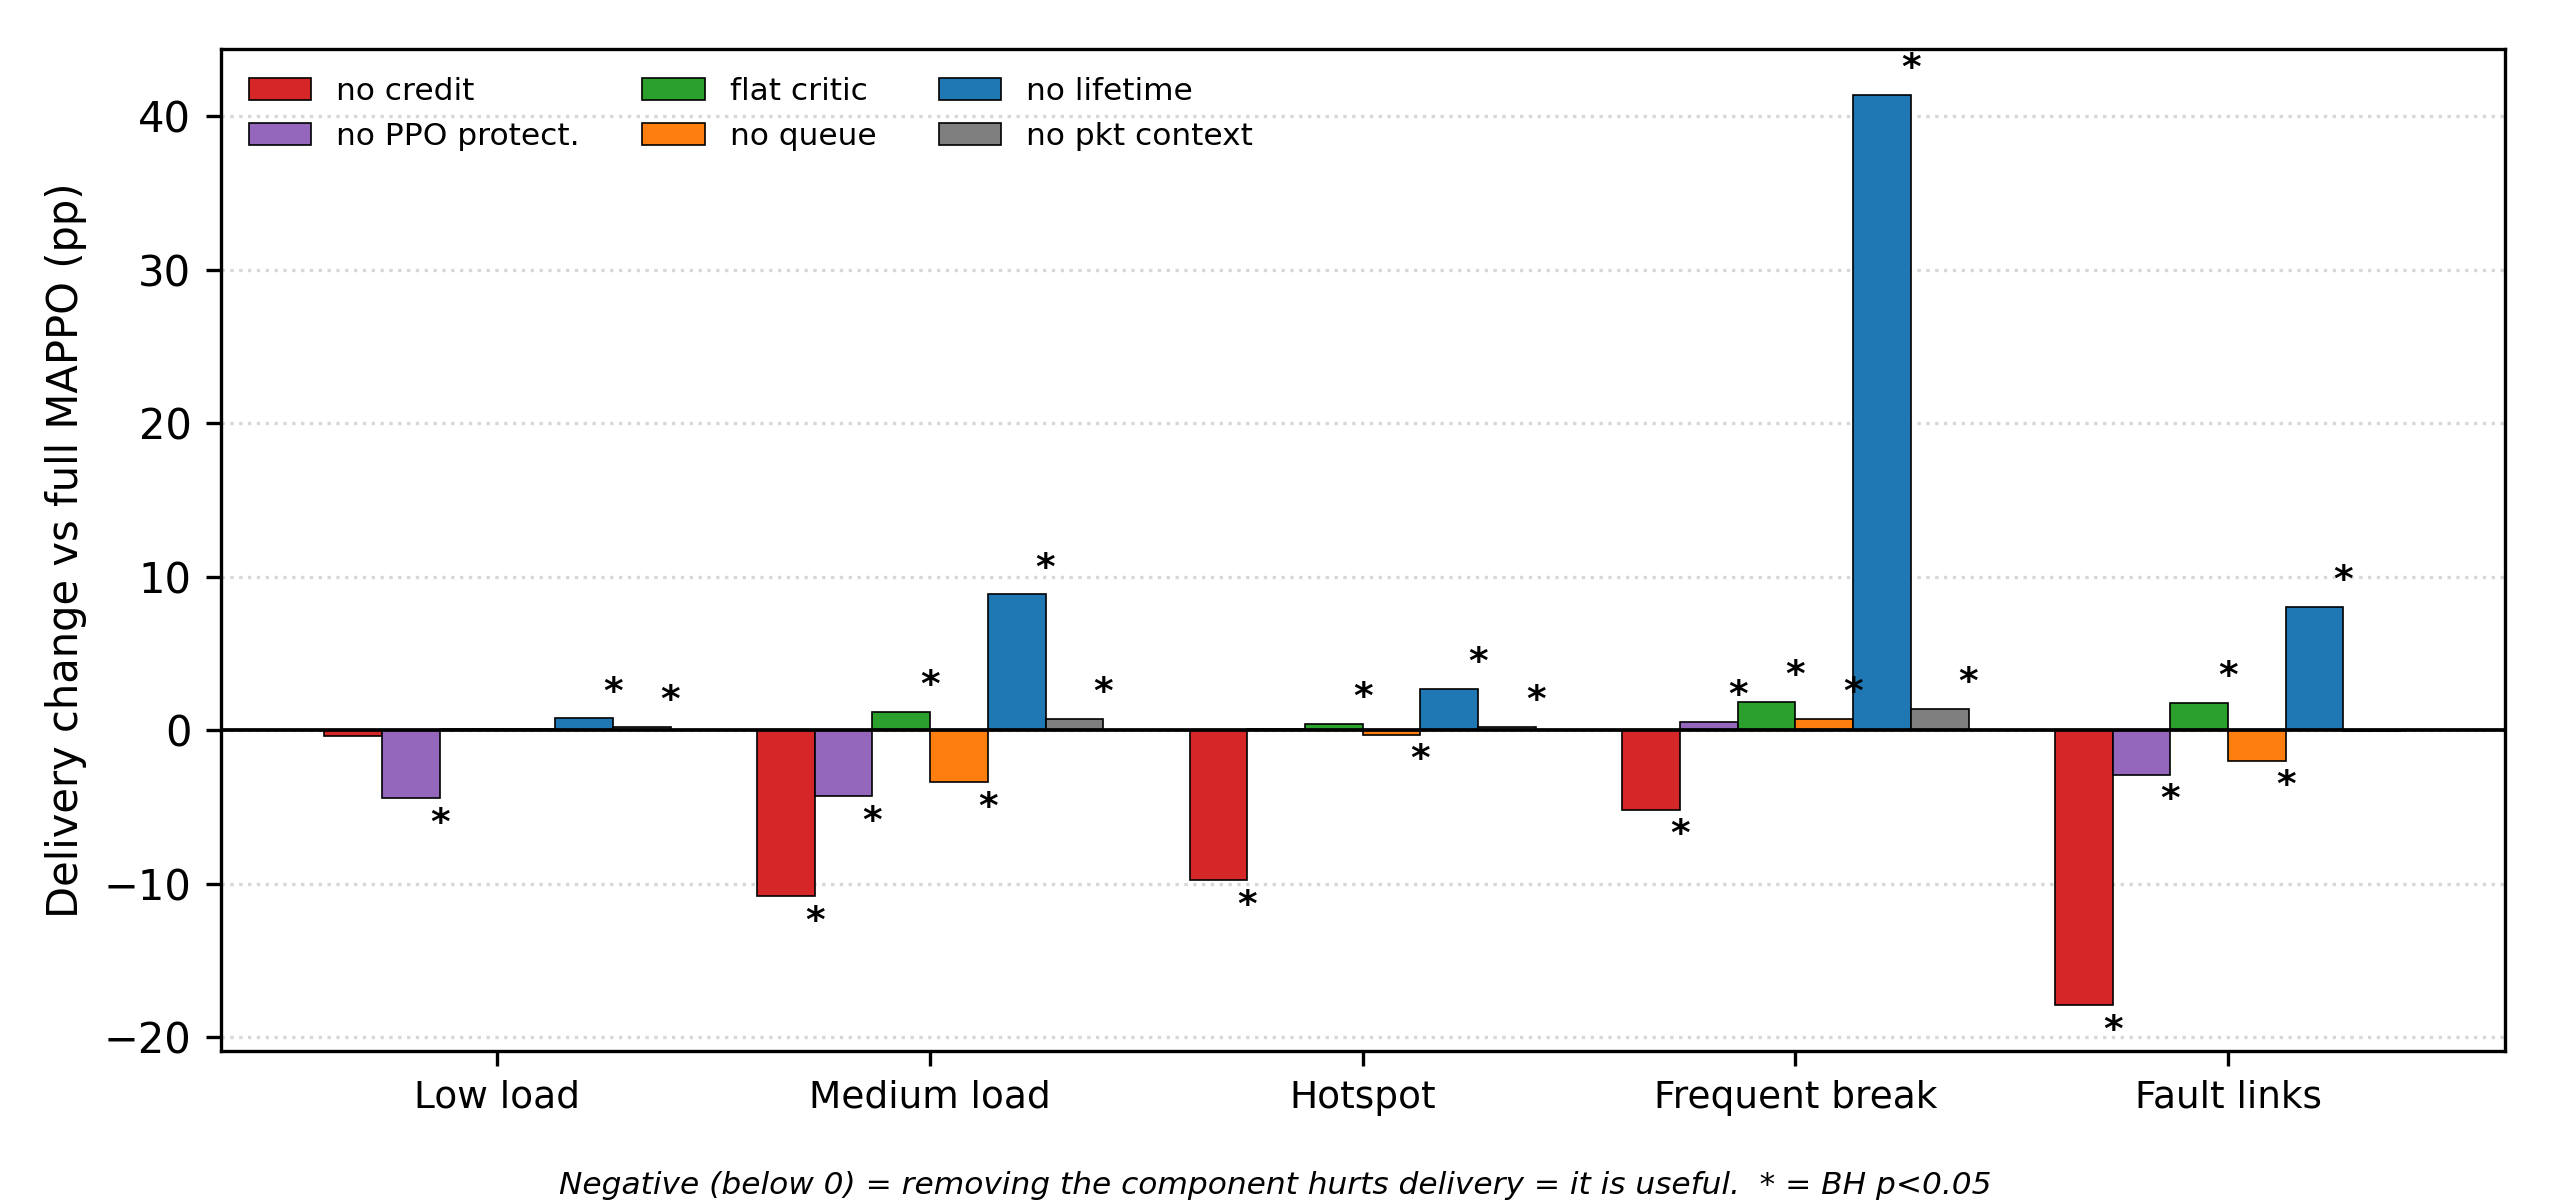
\includegraphics[width=\linewidth]{fig4_ablation_effect.png}
  \caption{Ablation effect (ablated minus full, in percentage points) across scenarios. Bars left of zero mean removing the component \emph{helps}; $\star$ marks Benjamini--Hochberg $p<0.05$. The lifetime subsystem is net-harmful (removing it helps everywhere); removing local credit is the most damaging.}
  \label{fig:ablation}
\end{figure}

\subsection{Sample efficiency and the budget--performance crossover}
\label{sec:budget}
A natural concern is whether the result is an artifact of a large training budget. Figure~\ref{fig:budget} traces mean delivery against training steps. The learned policy surpasses Q-routing and the queue-aware heuristic within 2\,k steps---well before convergence---and reaches the centralized-oracle band by 50\,k. The crossover is monotone across all five scenarios. This converts a potential reproducibility objection (``the policy needs a huge budget'') into a characterized sample-efficiency result: \emph{distributed-dominance is cheap; approaching the oracle is what costs budget.}

\begin{figure}[t]
  \centering
  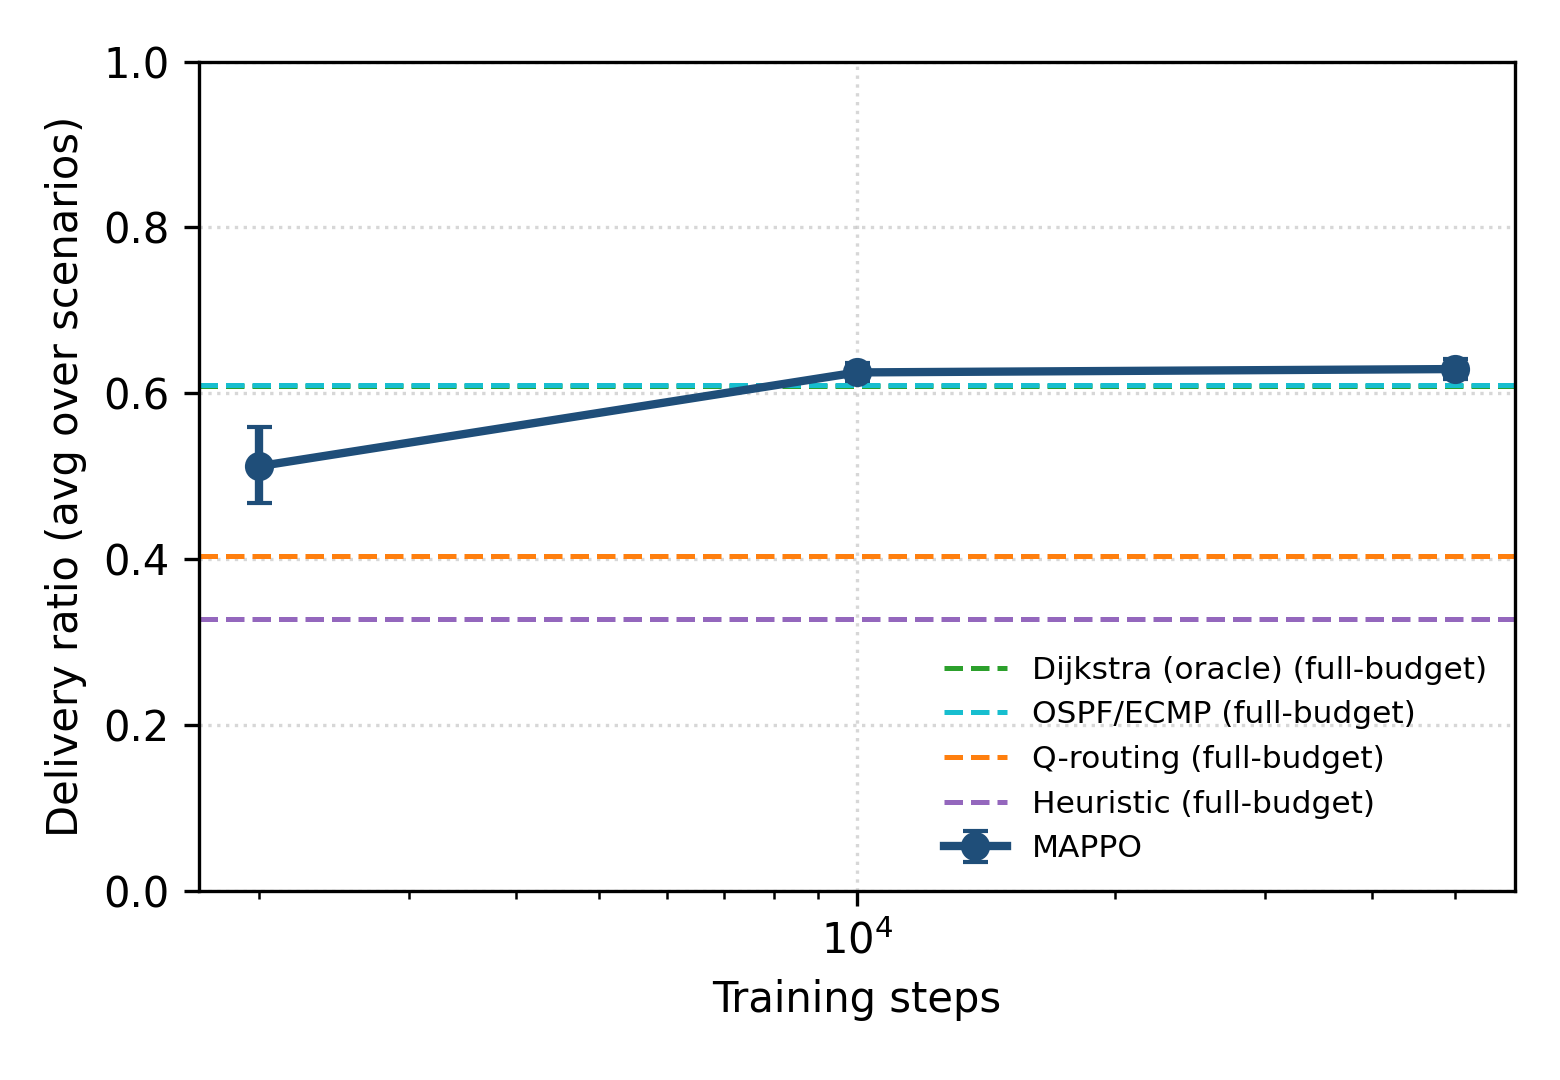
\includegraphics[width=\linewidth]{fig1_delivery_vs_budget.png}
  \caption{Delivery vs.\ training steps (mean over scenarios, 95\% intervals). MAPPO crosses the distributed baselines (Q-routing, heuristic) before 2\,k steps and converges to the Dijkstra/ECMP oracle band by 50\,k. (Dijkstra and ECMP overlap at the aggregate level.)}
  \label{fig:budget}
\end{figure}

\subsection{Cross-constellation transfer (C3)}
To test whether the policy learned routing competence rather than memorizing a specific topology, we take a policy trained on the primary Walker shell and evaluate it zero-shot on a different constellation geometry, with no fine-tuning. The transfer incurs a bounded delivery gap ($\approx -7.6$\,pp), demonstrating that the shared, permutation-equivariant policy carries over meaningful forwarding behavior across geometries. Both transfer directions were evaluated.

\subsection{Packet-level \texttt{ns-3} validation}
\label{sec:ns3}
We validate the policy in a packet-level \texttt{ns-3} simulation with injected ISL outages, using domain-adapted observations so the trained actor can drive the simulator directly. We report this as \emph{deployment-oriented} validation: it confirms the policy's behavior under a realistic packet scheduler and loss model, not identical-semantics transfer from the training simulator. The current fixture uses a smaller constellation; scaling to the full 24-satellite Starlink-shell fixture with 100+ injected drops is in progress and will be reported in the camera-ready version. We are explicit about this topology mismatch as a limitation.

% =============================================================================
\section{Discussion and Limitations}
\label{sec:discussion}
% =============================================================================

\textbf{On the comparison framing.} MAPPO does not comprehensively beat global Dijkstra on raw delivery, and we do not claim it does: the comparison is decentralized-versus-centralized and is favorable precisely because the local policy closes most of the information gap. The headline claims require the full training budget; we state the minimum (2\,k steps for distributed dominance, 50\,k for the oracle band).

\textbf{Confounding checks.} Delay is always reported alongside delivery to avoid survivor bias (shorter paths imply both higher delivery and lower delay only if the policy is not cherry-picking). Queue gains are reported against distributed baselines---the centralized oracles already achieve low queue, so the queue result is a tail/balance statement, not a delivery statement.

\textbf{Limitations.} (i) Eight policy seeds suffice for the paired tests reported, but a reviewer may demand more; we report policy-seed dispersion separately and provide MDEs on nulls. (ii) The \texttt{ns-3} validation uses a domain-adapted observation mapping and a smaller fixture than the training topology; full closed-loop validation on a matched 24-satellite fixture is in progress. (iii) The cross-constellation study uses real SGP4 positions but assumes simplified ISL geometry, capacity, and reliability; a full physical-layer ISL model is future work. (iv) The lifetime-subsystem negative result is, we believe, correct and robust (consistent across scenarios and metrics), but it is specific to our link-failure process; constellations with harder, less-predictable failures may benefit from a softened lifetime signal.

% =============================================================================
\section{Conclusion}
% =============================================================================

We showed that a distributed next-hop routing policy trained with shared-parameter MAPPO under CTDE---using only each satellite's queue state and one-hop neighbor information---can approach centralized shortest-path oracles to within a couple of percentage points on delivery while decisively dominating distributed baselines, and can do so with better tail latency and load balance where it matches the oracle. The result hinges on zero-mean local credit assignment, which the ablation isolates as the dominant architectural factor, and on disciplined PPO stabilization. An honest negative result---our intuitively-motivated link-lifetime mechanism proved harmful and was removed---underscores that even sensible components must be validated. Future work targets fully dynamic topologies, a matched-geometry \texttt{ns-3} closed loop, and larger constellations.

% =============================================================================
\bibliographystyle{IEEEtran}
\begin{thebibliography}{10}

\bibitem{yu2022surprising}
C.~Yu, A.~Velu, E.~Vinitsky, \emph{et al.}, ``The surprising effectiveness of PPO in cooperative multi-agent games,'' in \emph{Proc. NeurIPS Datasets and Benchmarks}, 2022.

\bibitem{leorl2023}
Authors, ``Queue-aware reinforcement learning for LEO satellite routing,'' \emph{arXiv:2306.01346}, 2023.

\bibitem{boyan1994q}
J.~Boyan and M.~Littman, ``Packet routing in dynamically changing networks: A reinforcement learning approach,'' in \emph{Proc. NeurIPS}, 1994.

\bibitem{hypatia}
S.~Kassing \emph{et al.}, ``Hypatia: Super-resolution modeling for high-fidelity LEO simulation,'' in \emph{Proc. ACM IMC}, 2020.

\bibitem{zaheer2017deep}
M.~Zaheer \emph{et al.}, ``Deep sets,'' in \emph{Proc. NeurIPS}, 2017.

\end{thebibliography}

\end{document}
